\documentclass[11pt, openright]{Thesis}      % Use the "Thesis" style, based on the ECS Thesis style by Steve Gunn
%\setpapersize{USletter}
\graphicspath{{Figures/}}  % Location of the graphics files (set up for graphics to be in PDF format)
% Include any extra LaTeX packages required
\usepackage[square, numbers, comma, sort&compress]{natbib}  % Use the "Natbib" style for the references in the Bibliography
\usepackage{verbatim}  % Needed for the "comment" environment to make LaTeX comments
\usepackage{vector}  % Allows "\bvec{}" and "\buvec{}" for "blackboard" style bold vectors in maths
\usepackage{color}
\usepackage{multirow} 
\usepackage{array}
%\usepackage[spanish,onelanguage]{algorithm2e}

\usepackage[english]{babel}
\usepackage[utf8]{inputenc}
\usepackage{tikz}
\usepackage{pgfgantt}
\usepackage{mathtools}
\usepackage{float}
\usepackage{tocstyle}
\usepackage{longtable}
\usepackage{rotating}
\usepackage{adjustbox}
\usepackage{booktabs}
\usepackage{hyperref}
\usetikzlibrary{matrix,chains,positioning,decorations.pathreplacing,arrows,fit}
\hypersetup{
    colorlinks=true,
    linkcolor=blue,
    filecolor=magenta,      
    urlcolor=blue, 
}
 
\urlstyle{same}
%% ----------------------------------------------------------------
\begin{document}
\frontmatter	  % Begin Roman style (i, ii, iii, iv...) page numbering

\begin{titlepage}

\newcommand{\HRule}{\rule{\linewidth}{0.5mm}} 

\center 


\includegraphics[scale=0.7]{Figures/logo_javeriana.pdf}\\[1cm] 

\textsc{\Large Research Proposal}\\[0.5cm] 

\HRule \\[0.4cm]
{ \huge \bfseries Artificial data generation to train object detection deep learning models: A case study in Banana diseases detection}\\[0.4cm] 
\HRule \\[1.5cm]

\begin{minipage}{0.4\textwidth}
\begin{flushleft} \large
\emph{Author:}\\
Javier Alejandro Vergara
\end{flushleft}
\end{minipage}
~
\begin{minipage}{0.4\textwidth}
\begin{flushright} \large
\emph{Director:} \\
Animesh Acharjee, PhD\\ 
\emph{Co-Director:} \\
Michael Selvaraj, PhD 
\end{flushright}

\end{minipage}\\[2cm]
\textbf{ Electronics and computer sciences
department}\\
\textbf{Pontificia Universidad Javeriana Cali}
\\
\vspace{5mm} %5mm vertical space
{\large \today}\\[2cm] 

\vfill 

\end{titlepage}

\pagestyle{fancy}  %The page style headers have been "empty" all this time, now use the "fancy" headers as defined before to bring them back
\usetocstyle[tocgraduated]{allwithdot}

%% ----------------------------------------------------------------
\tableofcontents  % Write out the Table of Contents

%% ----------------------------------------------------------------
\listoffigures  % Write out the List of Figures

%% ----------------------------------------------------------------
\listoftables  % Write out the List of Tables

%% ----------------------------------------------------------------
\acknowledgements
{
El autor agradece la cooperación de todos los miembros de la alianza \textit{Centro de Excelencia y Apropiaci\'{o}n en Internet de las Cosas (CEA-IoT)}. El autor agradece también a todas las instituciones que soportaron este trabajo: el \textit{Ministerio de Tecnolog\'{i}as de la Informaci\'{o}n y las Comunicaciones - MinTIC} y el \textit{Departamento Administrativo de Ciencia, Tecnolog\'{i}a e Innovaci\'{o}n - Colciencias} a través del \textit{Fondo Nacional de Financiamiento para la Ciencia, la Tecnolog\'{i}a y la Innovaci\'{o}n Francisco Jos\'{e} de Caldas} (Proyecto FP44842-502-2015).
}

%% ----------------------------------------------------------------
\setstretch{1.5}  % Set the line spacing to 1.5, this makes the following tables easier to read
\clearpage  % Start a new page
\listofsymbols{ll}  % Include a list of Abbreviations (a table of two columns)
{
\textbf{AMBA} & \textbf{A}dvanced \textbf{M}icrocontroller \textbf{B}us \textbf{A}rchitecture\\
\textbf{ANN} & \textbf{A}rtificial \textbf{N}eural \textbf{N}etwork \\
\textbf{AXI} & \textbf{A}dvanced e\textbf{X}tensible \textbf{I}nterface\\
\textbf{BRAM} & \textbf{B}lock \textbf{R}andom \textbf{A}ccess \textbf{M}emory\\
\textbf{DSP} & \textbf{D}igital \textbf{S}ignal \textbf{P}rocessor\\
\textbf{FF} & \textbf{F}lip \textbf{F}lop\\
\textbf{FPGA} & \textbf{F}ield \textbf{P}rogrammable \textbf{G}ate \textbf{A}rray\\
\textbf{HDL} & \textbf{H}ardware \textbf{D}escription \textbf{L}anguage \\
\textbf{HLS} & \textbf{H}igh \textbf{L}evel \textbf{S}ynthesis \\
%tek La siguiente línea marca un error
\textbf{IoT} & \textbf{I}nternet \textbf{o}f \textbf{T}hings\\
%\textbf{IoT} & \textbf{I}nternet of \textbf{T}hings\\
\textbf{IP} & \textbf{I}ntellectual \textbf{P}roperty\\
\textbf{LUT} & \textbf{L}ook \textbf{U}p \textbf{T}able\\
\textbf{MLP} & \textbf{M}ulti \textbf{L}ayer \textbf{P}erceptron \\
\textbf{OS} & \textbf{O}perating \textbf{S}ystem\\ 
\textbf{PL} & \textbf{P}rogrammable \textbf{L}ogic \\
\textbf{PS} & \textbf{P}rocessing \textbf{S}ystem \\
\textbf{QoS} & \textbf{Q}uality \textbf{o}f \textbf{S}ervice\\
\textbf{RTL} & \textbf{R}egister \textbf{T}ransfer \textbf{L}anguage\\
\textbf{SoC} & \textbf{S}ystem \textbf{o}n a \textbf{C}hip \\
\textbf{TDP} & \textbf{T}hermal \textbf{D}esign \textbf{P}ower
}

%% ----------------------------------------------------------------
% End of the pre-able, contents and lists of things

\mainmatter	  % Begin normal, numeric (1,2,3...) page numbering
\pagestyle{fancy}  % Return the page headers back to the "fancy" style

% Include the chapters of the thesis, as separate files
% Just uncomment the lines as you write the chapters
\singlespace


\chapter*{Abstract}

In Banana, early pests and diseases diagnosis is a crucial point due to most of these problems can be managed if they are early detected, pests and diseases affect a significant percentage of yield and food production this threat the local and global food security. New technologies are called to generate useful tools in the early diagnosis and disease detection tasks. Mobile applications with artificial intelligence and deep learning utilities could lead farmers in these tasks, but to train deep learning models is needed larger data sets which are not easy to generate, data augmentation techniques and artificially generated images are a good idea to face poor data problems. The goal of this proposal is to evaluate traditional data augmentation and artificial data generation techniques to increase the performance in deep learning models.

\providecommand{\keywords}[1]
{
  \small	
  \textbf{\textit{Keywords---}} #1
}

\keywords{Deep learning, generative adversarial networks, artificial data, data augmentation, transfer learning} % Abstract
\chapter{Introduction} % Write in your own chapter title
\label{Chapter1}
\lhead{Chapter 1. \emph{Introduction}}

In agriculture there are several environmental threats as drought, pest, and diseases, nutrient deficiency, etc. that affects the crops, reduce their yield and decrease food production. Farmers around the world have the challenge to face those problems, but they do not have enough tools to do it because for years there has been a gap between technology and agriculture. Some few organizations have the power and the technology to make its crops resistant to many threats, but 85\% of the world’s farms are in smallholder farmers hands\cite{nagayets2005small}. Smallholder farmers rely on empirical knowledge, which is less effective in this overcoming farming challenges\cite{hillnhuetter2008early}, technology must be closer to them and enrich their knowledge to improve their food production. 

One good example is Banana, Banana is one of the most important fruit crops in the world  in terms of production volume and trade\cite{faostat2014food}. Only a low percentage of bananas produced are globally traded\cite{lescot2013world}, most of the production is for domestic markets, this crop is a substantial dietary component \cite{abele2007bacterial} due to the nutritional facts and in some countries as Colombia a lot of typical dishes are made from this fruit.
But as mentioned several pests and diseases affect banana crops causing significant yield losses\cite{blomme2017bacterial}, most of these diseases are presented as physical symptoms specially in leaves and if this is not controlled, pests and diseases will affect the whole crop and even the surrounding farms, an early detection system is needed to help farmers to manage those threats. Also, there are many concerns about the change and the increase of those problems due to climate change\cite{garrett2013cambio}\cite{hamada2011impacts}. To help not only banana farmers but all crops and to close the gap between the agriculture and technology, different areas in science are called to create and develop useful and low-cost technological tools applied to agriculture and easy to use for smallholder farmers to help them with all those threats. Some examples are mobile applications \cite{qiang2012mobile} , crop monitoring\cite{berni2009thermal}\cite{hunt2010acquisition}, Internet of thing(IoT)\cite{baoyun2009review} , remote sensing\cite{doraiswamy2003crop} and artificial intelligence \cite{murase2000artificial}. 
Artificial intelligence(AI) and specifically machine learning and deep learning applications are helping in disease detection in humans 
\cite{esteva2017dermatologist}, \cite{rajpurkar2017chexnet} , \cite{shen2017deep}  but also in plants \cite{mohanty2016using} and combined with mobile applications are becoming into great tools in crop diagnosis and management\cite{ramcharan2017deep}. Deep learning models can be trained with different sources of data, but in diseases diagnosis image based\cite{mohanty2016using} models are used since diseases symptoms are clearly observable. The major problems in machine learning and specially in deep learning applications are the source of information, due to these networks require a massive amount of data to be trained and perform a good generalization, is not easy to obtain a good database with reliable and enough data. As disease diagnosis with deep learning use images, there are some traditional methods to do data augmentation such as flipping or mirroring the images \cite{bloice2017augmentor}, but new technologies are coming to generate artificial images with an approach called generative adversarial networks(GAN)\cite{NIPS2014_5423} \cite{perez2017effectiveness} , with these models can be generated artificial data almost real and makes impossible to differentiate between a real and an artificial image for human been\cite{karras2018style}.

Data augmentation with traditional and new techniques are giving solutions to poor data problems and helps to increase the accuracy of the trained models\cite{barbedo2018impact}. To develop this study, context and planning is organized in 8 sections as follows:
\begin{itemize}
\item Section two for the possible title of the final work.
\item Section three and four contents the problem description, the scope of this work within that context and the objectives. 
\item Section five sets the reasons and the importance to conduct this project.
\item Section six is a brief of the state of the art and the theoretical basis for the starting steps.
\item Section seven and eight describes how will be executed this work and establish each step of the process, the activities and the resources needed.
\end{itemize} % Introducción
% Chapter 2

\chapter{Problem formulation} % Write in your own chapter title
\label{Chapter2}
\lhead{Chapter 2. \emph{Problem formulation}} % Write in your own chapter title to set the page header

Climate change, pest, and diseases and all the environmental phenomena that currently affect the world, have generated different challenges to deal in the incoming years. One of those challenges is the direct impact on food security \cite{wheeler2013climate} at a global level; this has called attention at a global scale to generate  resistant crops to all these factors and at same time increasing yield and its nutritional value (plant breeders tasks) but also giving tools to farmers to increase and warrant their food production.

One selected important crop to face the food security problem is Banana \textit{(Musa spp)}\cite{faostat2014food};
Though a major staple in Africa, Asia, and Latin America, only 13\% of bananas produced are globally traded \cite{lescot2013world}, clearly indicating the fruit’s importance in domestic markets and for food security. In East and Central Africa, it is a substantial dietary component, accounting for over 50\% of daily total food intake in parts of Uganda and Rwanda\cite{abele2007bacterial}. In Colombia, Banana is one of the main fruit crops that sustain the country's food security and it as a part of different typical dishes.

A big concern in Banana are pest and diseases, and this has a direct impact on yield and food production. Several diseases affect banana crops around the world threaten food security, such as Banana bunchy top virus(BBTV), banana Xanthomonas wilt(BXW)(see figure \ref{fig:subim1}), Black and Yellow Sigatoka and Fusarium wilt and some pest as Banana Weevil(see figure \ref{fig:subim2}). In order to manage the spread of crop diseases and pest, early identification in the field is a crucial step. Fortunately, most of the crop diseases can be managed by detecting the diseases as soon as it appears on the crop. Traditional pest and disease identification approaches rely on the support of agricultural extension specialists, but these approaches are limited in developing countries with low human infrastructure capacity. The major part of banana crops around the world are from smallholders farmers; they do not know, or they use empirical methods to make the diagnosis, but the early identification of the problem is not possible in most of the cases. 



\begin{figure}[H]
     \centering
     \begin{subfigure}[b]{0.3\textwidth}
         \centering
         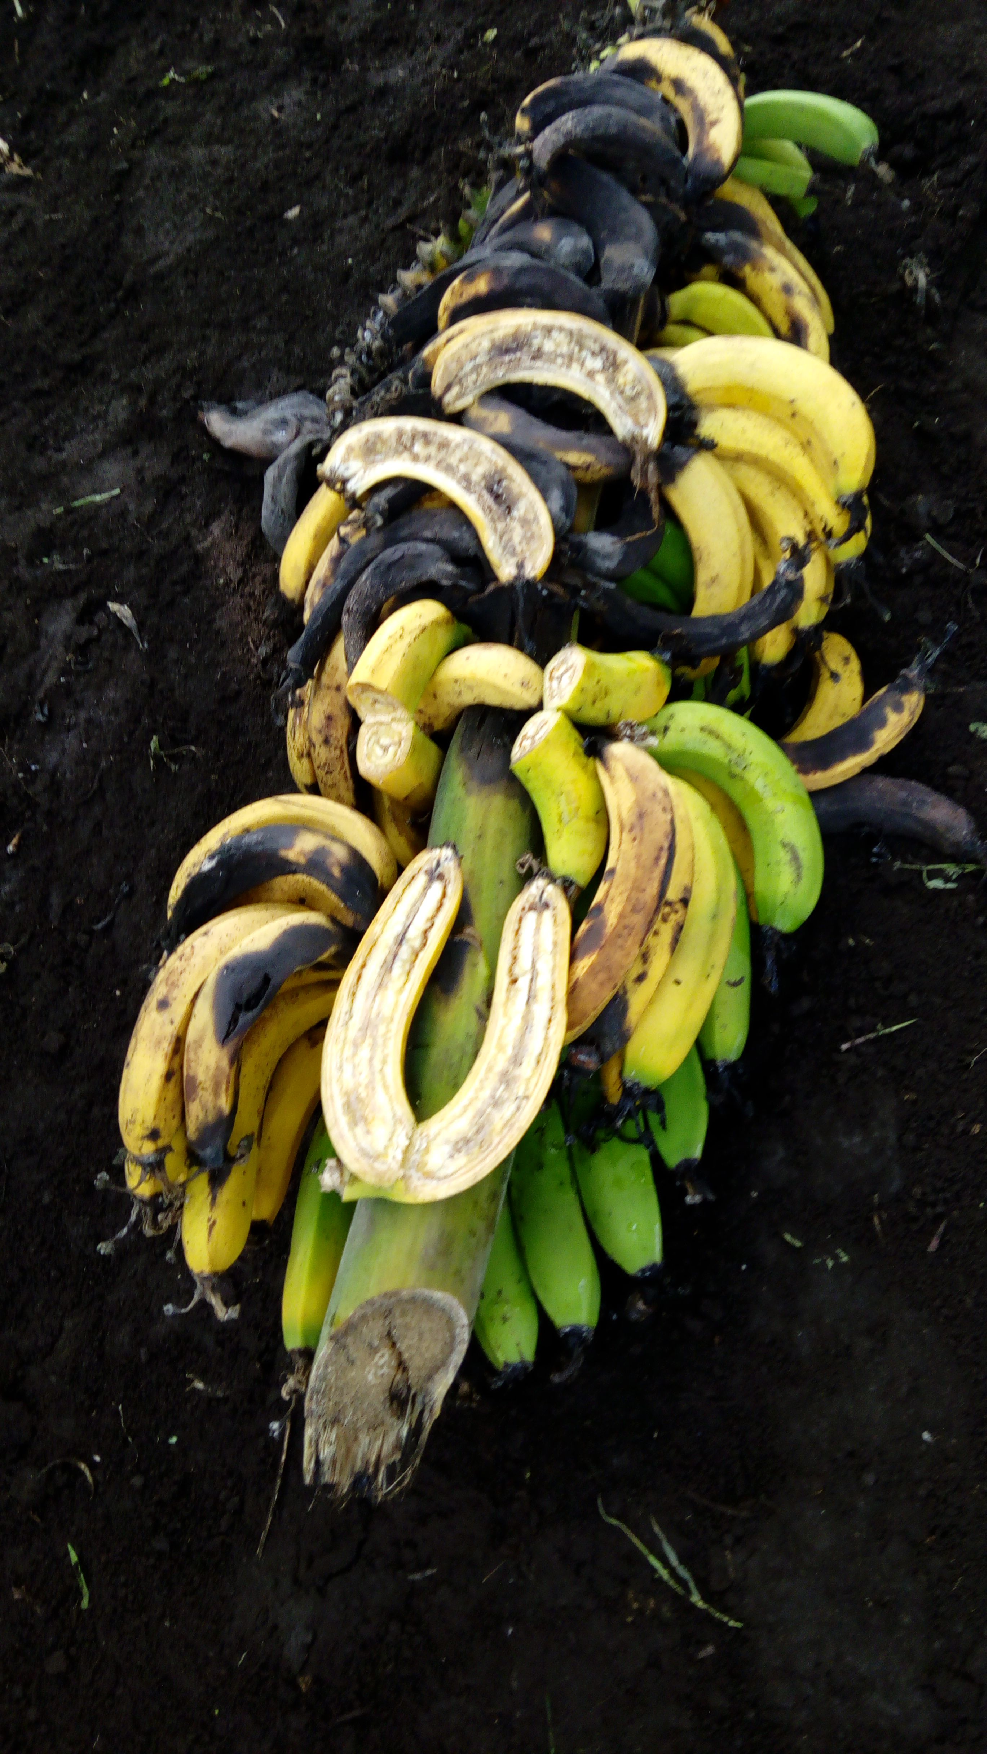
\includegraphics[width=0.9\linewidth, height=5cm]{Figures/bunch.pdf} 
         \caption{BXW in banana fruit bunch}
         \label{fig:subim1}
     \end{subfigure}
     \hfill
     \begin{subfigure}[b]{0.3\textwidth}
         \centering
         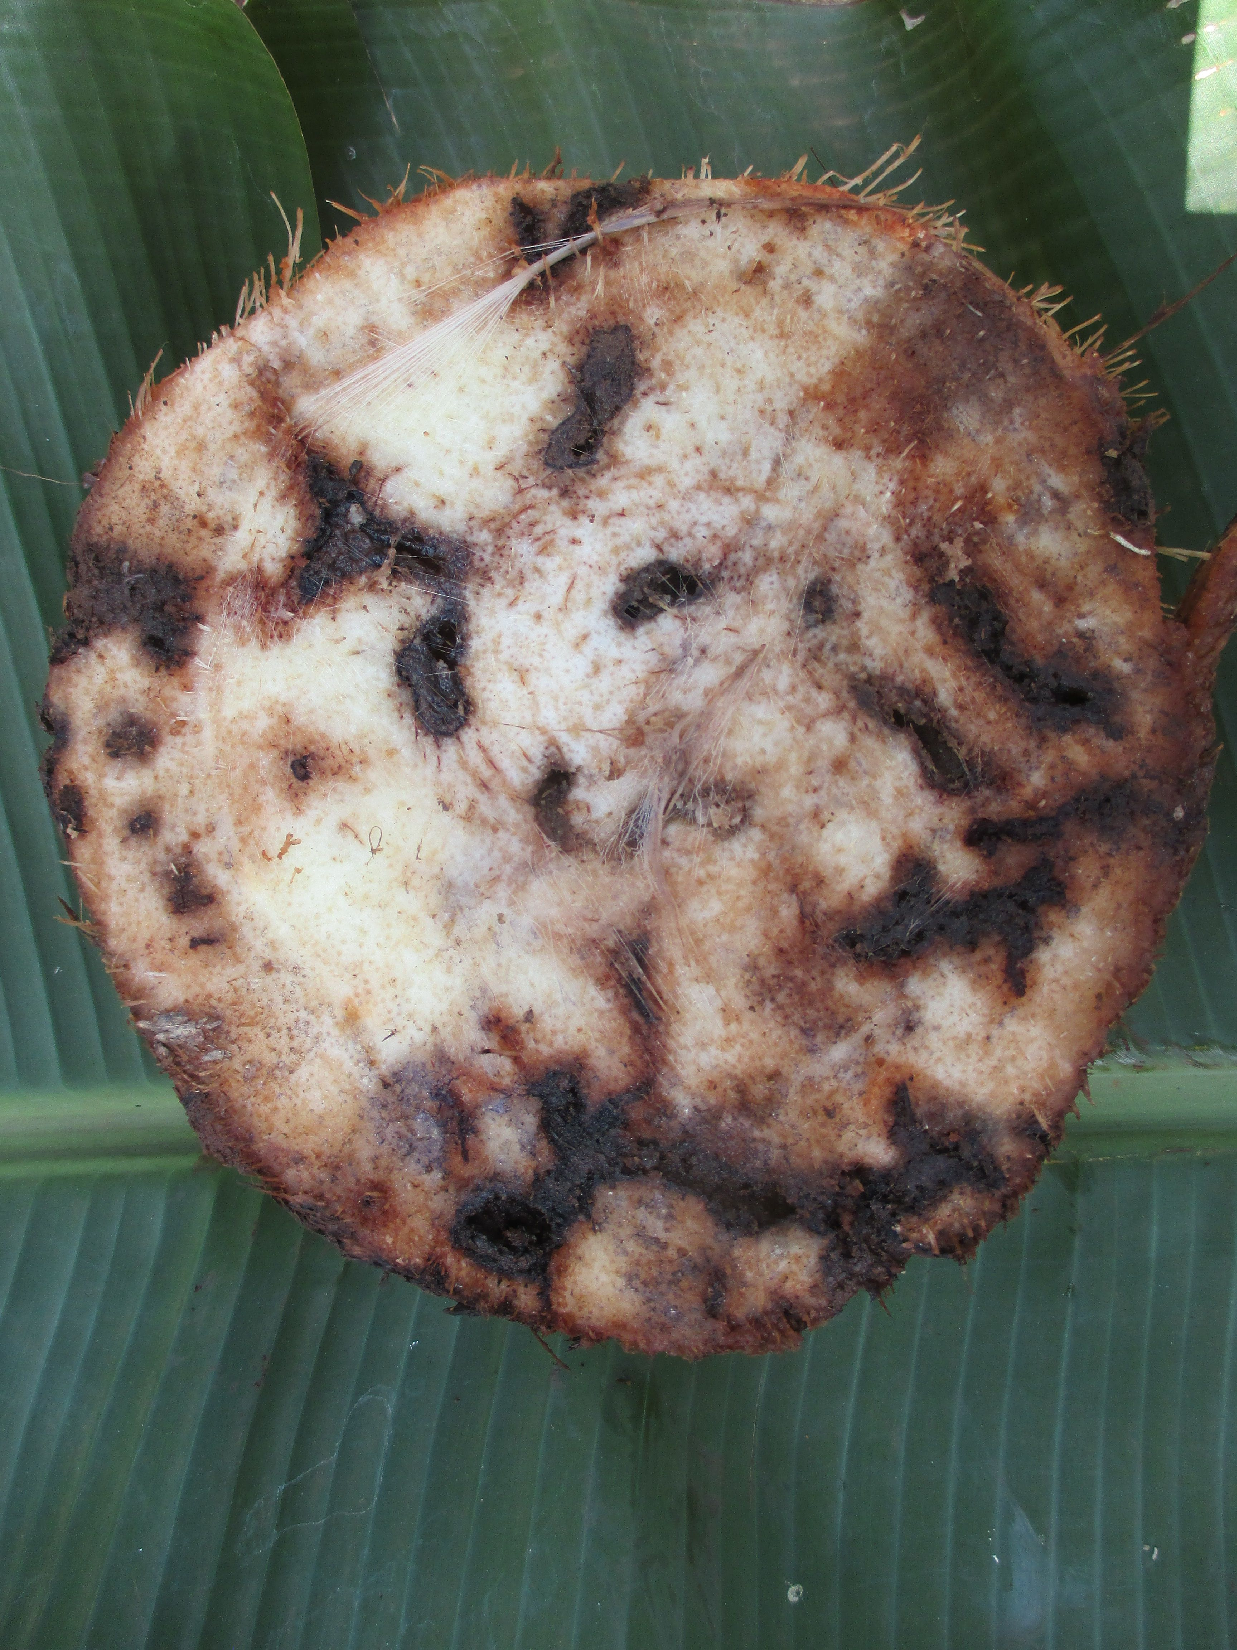
\includegraphics[width=0.9\linewidth, height=5cm]{Figures/corm.pdf}
         \caption{Banana weevil effects in the corm}
         \label{fig:subim2}
     \end{subfigure}
     \hfill
        \caption{Disease and pest impact in banana}
        \label{fig:image2}
\end{figure}


Artificial intelligence (AI) with deep learning models \cite{goodfellow2016deep} are useful to help identify plant diseases by the plant’s appearance and visual symptoms\cite{camargo2009image}. Deep learning models can be embedded in smartphones to create applications that could alert farmers of the presence of a disease, lead to concerted control actions and thus potentially preventing a disease from spreading over large areas\cite{mohanty2016using}. Even though many of the developing country farmers around the world do not have access to these advanced tools, internet infiltration and smartphone penetration offer new outfits for in-field crop disease detection. The GMSA (Global System for Mobile Association) predicted that global smartphone subscriptions would reach 5 billion by 2020, of which nearly one billion in Africa (GSMA Intelligence, 2016). 
Mobile applications are promising to be excellent tools to support farmers in disease detection and crop management. The main problem with AI applications is that it is needed vast amounts of data to train the models and have reliable predictions, since in deep learning techniques specially in object detection models the main data source are images, it also need many images to learn the patterns. In real cases is very difficult to obtain a data set with enough and reliable images, because the images should be taken in different environmental conditions, different hours (morning, noon and afternoon) and by disease experts. 

As banana is one of the most important fruit crops around the world, it is needed to create easy tools to detect diseases using deep learning models, but there is a big problem and is the data acquisition as mentioned before, fortunately, traditional data augmentation methods have demonstrated  to be an excellent option to increase the number of images\cite{barbedo2018impact} but these approaches are just making the models more robust to orientation using the same original information, so creating new artificial information is the real call of duty, generated artificial data could improve not only the performance of the deep learning models but the generalization capabilities, and this is the scope for this work. To evaluate if artificial data is strong enough and a good option in order to increase the accuracy and the performance of deep learning models but also to ease the creation of new technology implemented in Banana for the future, following research questions have been generated: 
\begin{itemize} 
\item Traditional data augmentation techniques are enough to increase the performance of object detection deep learning models in banana disease detection?
\item Artificial data helps in disease diagnostic tasks?
\item How many images are needed to have a good performance in object detection deep learning models for banana diseases?
\item Combining real data with augmentation techniques and artificial data will improve the performance of object detection deep learning models?
\end{itemize}   % Definición del Problema 

%\chapter{Scope} % Write in your own chapter title
\label{Chapter3}
\lhead{Chapter 3. \emph{Scope}} % Write in your own chapter title to set the page header

The scope of this work is to apply traditional data augmentation and artificial data generation techniques to asses the performance of object detection deep learning models in banana disease detection tasks. It aims to:

\begin{itemize}
\item To create a banana diseases data set to train object detection deep learning models 
\item To evaluate traditional and novel techniques for data augmentation 
\item To compare the performance of object detection deep learning models using real, artificial and combined data. 
\item To document the workflow and the results of this work    
\end{itemize} % Objetivos 

%\chapter{Objetives} % Write in your own chapter title
\label{Chapter4}
\lhead{Chapter 4. \emph{Objetives}} % Write in your own chapter title to set the page header

\section{General Objective} 
To evaluate the performance of object detection deep learning models using traditional data augmentation and artificial data generation techniques in banana disease detection. 
\section{Specific Objectives} 
\begin{itemize} 
\item To create and label banana diseases data set
\item To train Generative adversarial networks to generate artificial banana diseases images
\item To generate two data sets of artificial images using traditional data augmentation techniques and GAN models
\item To train object detection deep learning models with the real, augmented, artificial and combined data sets
\item To evaluate and compare the performance of the trained models.
\end{itemize}    % Justificación 

%\chapter{Justification} % Write in your own chapter title
\label{Chapter4}
\lhead{Chapter 4. \emph{Justification}}

Applying machine learning techniques such as deep learning and object detection, help farmers not only to diseases classification but detection, for instance, some diseases are presented just in the leaves so this approaches can tell to the farmer which disease and where is it. Fortunately, mayor banana diseases can be treated if are detected in early stages, for instance, mobile applications using deep learning models give a practical tool to the farmers for real in-field detection and additionally crop management advises controlling the current disease. Also, the geolocation information of the images can describe the behavior and the spreading of the diseases through a city or even a country. But the major problem that is not letting this technology going on to the future is the data acquisition. 

Data acquisition for training deep learning models is time-consuming, long duration, experts are required and a massive amount of images with several variations. So data augmentation techniques and artificial data generation as GAN models, have the duty to help in this task making these models more robust and increasing the performance. This study has the purpose of evaluating if GAN models as new artificial data generation technique have the power to generate quality data to take this information into account in deep learning training processes, if GAN models can generate such that quality data more real-world applications in future will be developed due to the capability of new data generation, helping farmers in their daily tasks, such as crop evaluation, providing them useful tools for early diagnosis and disease detection

Farmers have been distant to novel technologies for years, getting those technologies close to them as in this study, reducing the number of images to be acquired to train deep learning model, making the job easier to create useful technology that in the incoming years will contribute to food security.
With the improvement of all these things and technological support can be faced food security problems in the future because with the development of early diagnosis tools and more mobile applications for farmers, they can be lead to have better yield, improve their food production and raise their gains warranting the local food needs. Giving them technological support to face those problems and to improve their crops, making them closer to new technologies and creating tools is an excellent way to make the world more sustainable. % Alcances 

%\chapter{Marco Teórico} % Write in your own chapter title
\label{Chapter6}
\lhead{Capítulo 6. \emph{Marco Teórico}}

\section{Theoretical framework}

\subsection{State of the art}
\subsubsection{Automatic Plant diseases detection}

Plant disease classification is a very complex task as it relies on experts hands, but there are some automatic systems for the automatic detection of diseases, image processing, machine learning, and deep learning are some use-full tools to help in these tasks (see figure \ref{fig:detec}). Up to now most of the approaches for plant disease detection were depending on machine learning algorithms, these approaches are easily adapted to certain conditions as light for instance,  if the system has a new input with a tiny variation the accuracy of the model will decrease\cite{inbook}. The development of deep learning, deeper networks, convolutional neuronal networks (CNN) and transfer learning approach creates new models that are not as susceptible as common machine learning techniques.
\begin{figure}[h]
\centering
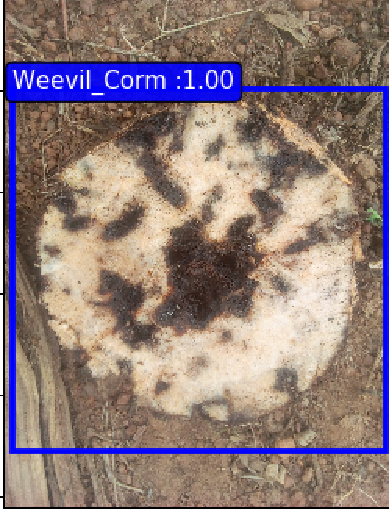
\includegraphics[scale=0.6]{Figures/result1.pdf}
\caption{Automatic pest detection in Banana using deep learning}
\label{fig:detec}
\end{figure}

\subsubsection{Pattern recognition}

Pattern recognition is a big knowledge area and is used in several applications in real life such as modelling, data management, commerce and even in politics. Disease diagnosis and detection are important topics to explore with pattern recognition and they have shown good results\cite{zhang2013nmr,felson1979new} also with techniques as machine learning\cite{kononenko2001machine,sajda2006machine}. Recently all these techniques are being applied in agriculture applications, starting with crop modeling \cite{bannayan2009using} , using support vector machines for crop classification \cite{camps2003support} and for plant disease detection \cite{rumpf2010early}.

\subsubsection{Deep learning}

Starting from machine learning networks, the necessity to create robust models, capable to manage several training classes, great inference power and good performance, made machine learning networks to grow in the sense of these new networks are deeper. For example in the ImageNet challenge(2012), AlexNet had a good performance\cite{NIPS2012_4824}. deep learning networks are working in important areas as face detection and agriculture, being this last a promising field to apply those techniques. Deep learning is used in Plant stress phenotyping\cite{SINGH2018883}, Plant diseases and pests detection in tomato\cite{article} ,Cassava disease detection\cite{ramcharan2017deep}\cite{sladojevic2016neural}, finally deep learning can be embedded into smartphones to create useful applications helping with disease diagnosis\cite{ramcharan}.

\subsubsection{Object detection} 

Classification in deep learning tasks aims to predict a class inside an image, for instance, if it is wanted to differentiate between if what there are in the images is a cat or a dog, the model can predict which animal it is. Object detection not just classify between a cat or a dog but detects where inside the image is the detected object (see figure \ref{fig:Spectral_Signature}), in this way, the system may tell the farmer where the disease is in a real scenario\cite{article}.Two examples of this technology in a real scenario are in Cassava and tomato, where object detection and transfer learning were used to detect diseases in the cassava and tomato leaves\cite{ramcharan}\cite{article} and implemented as a mobile application\cite{ramcharan2017using}. Currently, convolutional Neural Networks (CNN) are considered as the foremost method for object detection and there are some well performed methodologies such as Faster R-CNN and Single Shot Detectors (SSD). The evaluation of the performance is different from classification techniques as confusion matrix, there are some techniques to do the evaluation as mean average precision (mAP) score.

\begin{figure}[h]
\centering
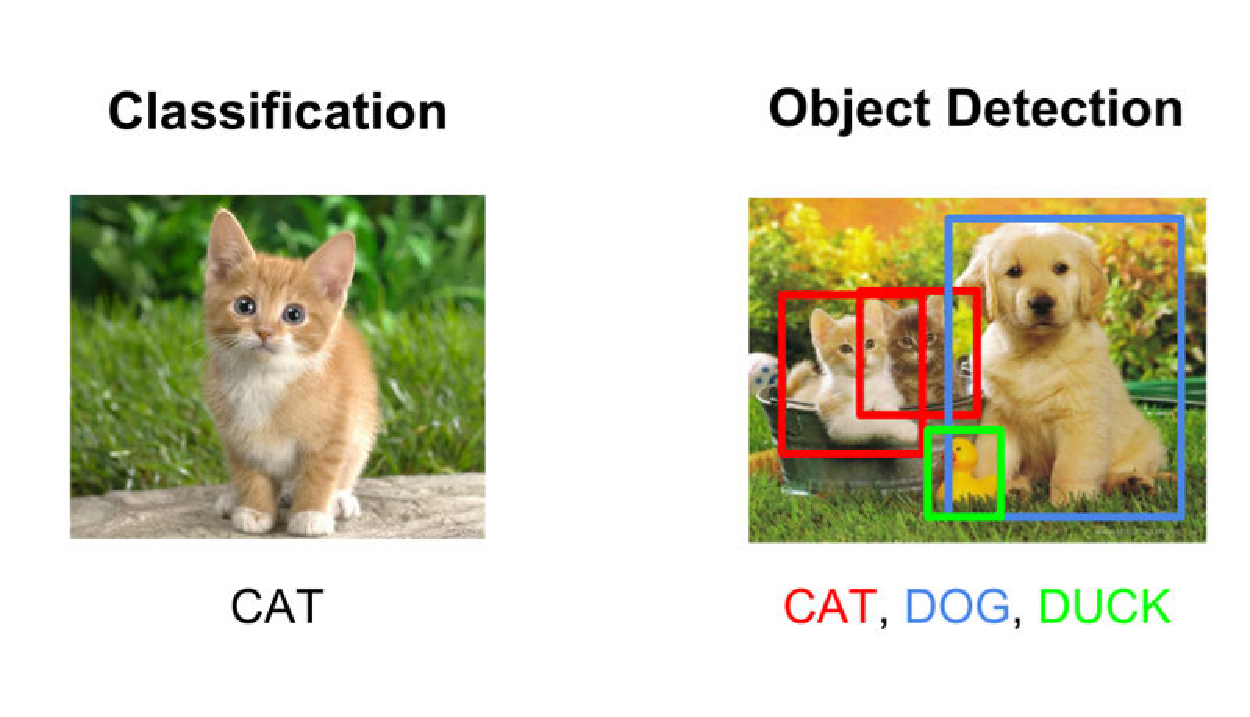
\includegraphics[scale=0.4]{Figures/object.pdf}
\caption{Difference between classification and object detection. From: Datacamp.[Online] Available at: https://www.datacamp.com/community/tutorials/object-detection-guide}
\label{fig:Spectral_Signature}
\end{figure}

\subsubsection{Transfer learning}

Transfer learning is becoming into an exciting way to face poor data situations \cite{pan2010survey}, is well known that for deep learning is needed huge data to train the network, what transfer learning is giving is a new technique to take pre-trained networks and adapt them to do a new task \cite{torrey2010transfer}. For instance, an existing network trained to classify cars can be re-trained to classify trucks without a training process from scratch, reducing the training time and getting faster results. 

\subsubsection{Generative adversarial networks}

GAN models are part of artificial intelligence, they are part of non supervising learning approaches which creates a system with two neuronal networks that compete with each other, were created by Ian Goodfellow et al. in 2014 \cite{NIPS2014_5423}. GAN models are currently being used in different applications: Style based generator architecture \cite{DBLP} that is a work from NVIDIA's team capable to generate artificial information based on two images and creating a new one with the mixing of features from both  images. Another  application is creating super resolution images\cite{DBLP1}. In conclusion, GAN models can generate artificial data to augment a data set to train deep learning models.

\subsubsection{Traditional data augmentation techniques}
Some machine and deep learning problems requires a data set with hundred or thousand of images, which is hard to collect in most of the cases, but with few images can be generate new samples to train the models applying different techniques\cite{barbedo2018impact} such as:
\begin{itemize} 
\item Vertical and horizontal flipping  
\item Image rotations
\item Brightness decrease and brightness increase
\item Contrast enhancement and contrast reduction
\item Sharpness enhancement
\item Addition of random Gaussian noise
\end{itemize}   

Those traditional techniques make models more robust and invariant to some variables as light condition and angle rotation, increasing the accuracy of the model. % Marco Téorico 

%\chapter{Recursos} % Write in your own chapter title
\label{Chapter7}
\lhead{Capítulo 7. \emph{Recursos}} % Write in your own chapter title to set the page header

\section{Human Resources}
\subsection{Director}
Dr. Animesh Acharjee, UK Centre for Computational Biology, University of Birmingham, UK.
\subsection{Co-Director}
Dr. Michael Gomez Selvaraj, International Center for Tropical Agriculture (CIAT), Palmira-Colombia.
\subsection{Consultants}
\begin{itemize}
\item PhD student Henry Ruiz, Texas A\&M University, Texas-United states.
\item MSc. Milton Valencia, International Center for Tropical Agriculture (CIAT), Palmira-Colombia.
\item MSc. Manuel Alejandro Valderrama, International Center for Tropical Agriculture (CIAT), Palmira-Colombia.
\end{itemize}
\subsection{Research Group}
International Center for Tropical Agriculture (CIAT)

\section{Budget}
\subsection{General Budget}
The general budget (Materials, inputs, equipments, software, hardware and bibliographic material)  for this work is shown in table \ref{table1} , This project is funded by CIAT programs

\begin{table}[h]
\centering

\begin{tabular}{l|l}
\hline
 \textbf{Item} & \textbf{Price (USD)}    \\ \hline
 Advisor& \$ 2000    \\
 Co-Advisor&  \$ 2000     \\
 Consultants& \$ 2000      \\
 Student&    \$ 8000   \\
 Bibliographic material & \$ 1000 \\
 Laptop&   \$ 1500    \\
 Software&  \$ 5000    \\
 Materials&   \$ 2000    \\ \hline \hline
 Subtotal&  \$ 23500     \\ 
 10\% Effort & \$ 2350      \\ \hline \hline
 Total&  \$   25850   \\ \hline \hline
\end{tabular}
\caption{\label{table1} General Budget}
\end{table} % Metodología 

%% Chapter 8
\chapter{Metodología} % Write in your own chapter title
\label{Chapter8}
\lhead{Capítulo 8. \emph{Metodología}} % Write in your own chapter title to set the page header


\section{Research Methodology}

This work is an analytic research to evaluate the performance of deep learning models trained with different sources of information (real and artificial data). 

\subsection{Activities}

To achieve the objective of this work and following each sub-objective, have been proposed the following probes and activities:\\

\textbf{Activity 1. To create and label real banana diseases data set}

\begin{enumerate}
    \item To collect banana images from different places.
    \item To filter the images.    
    \item To split and arrange the images in a structured format (Class based).
    \item To label the images with the correct bounding box and class label.
\end{enumerate}

\emph{Materials:}
\begin{itemize}
	\item Smartphone or RGB camera
    \item Laptop:\\Processor: Intel Core i7-6700HQ Quad Core Processor (6M Cache, 2.6GHz - 3.5GHz)\\Ram: 32GB RAM DDR4 2133MHz \\ Hard Drive: 500GB Solid State Drive + 2TB 5400rpm Hard Disk Drive \\ Graphics Card: NVIDIA GeForce GTX 960M 4GB
    \item Storage space
    \item Label image Software
\end{itemize}

\textbf{Activity 2. To train Generative adversarial networks generating artificial banana diseases images}

\begin{enumerate}
    \item To enrich the knowledge about GAN models
    \item To explore different GAN models.
    \item To select one GAN methodology and apply the methodology generating new data.    
    \item To test the quality of the generated data.
\end{enumerate}

\emph{Materials:}
\begin{itemize}
    \item Laptop:\\Processor: Intel Core i7-6700HQ Quad Core Processor (6M Cache, 2.6GHz - 3.5GHz)\\Ram: 32GB RAM DDR4 2133MHz \\ Hard Drive: 500GB Solid State Drive + 2TB 5400rpm Hard Disk Drive \\ Graphics Card: NVIDIA GeForce GTX 960M 4GB
    \item  Server: Processor: Intel Xeon E5-2667 v4 @ 3.20 GHz  x16, GPU: NVIDIA Tesla M60, OS: Windows Server 2016 x64 
    \item Python Software
    \subitem Numpy\subitem Scipy \subitem Pandas \subitem Matplotlib  \subitem Augmentor \subitem PyTorch \subitem Keras \subitem TensorFlow
\end{itemize}


\textbf{Activity 3. To generate two data sets of artificial images using traditional data augmentation techniques and GAN models}

\begin{enumerate}
	\item To select traditional data augmentation techniques.
	\item To apply the selected techniques to create the new data set.
	\item To create a data set with GAN artificial images.
	\item To label the images with the correct bounding box and class label .
\end{enumerate}
\emph{Materials:}
    \begin{itemize}
    \item Laptop:\\Processor: Intel Core i7-6700HQ Quad Core Processor (6M Cache, 2.6GHz - 3.5GHz)\\Ram: 32GB RAM DDR4 2133MHz \\ Hard Drive: 500GB Solid State Drive + 2TB 5400rpm Hard Disk Drive \\ Graphics Card: NVIDIA GeForce GTX 960M 4GB.
    \item Label image Software
\end{itemize}

\textbf{Activity 4. To train deep learning models with the real, augmented, artificial and combined data sets}

\begin{enumerate}
	\item To train deep learning models with real data.
	\item To train deep learning models with augmented data.
	\item To train deep learning models with artificial data.
	\item To train deep learning models with combined data.
\end{enumerate}
\emph{Materials:}
    \begin{itemize}
    \item Laptop:\\Processor: Intel Core i7-6700HQ Quad Core Processor (6M Cache, 2.6GHz - 3.5GHz)\\Ram: 32GB RAM DDR4 2133MHz \\ Hard Drive: 500GB Solid State Drive + 2TB 5400rpm Hard Disk Drive \\ Graphics Card: NVIDIA GeForce GTX 960M 4GB
    \item  Server: Processor: Intel Xeon E5-2667 v4 @ 3.20 GHz  x16, GPU: NVIDIA Tesla M60, OS: Windows Server 2016 x64 
    \item Python Software
    \subitem Numpy\subitem Scipy \subitem Pandas \subitem Matplotlib  \subitem Augmentor \subitem PyTorch \subitem Keras \subitem TensorFlow
\end{itemize}

\textbf{Activity 5. To evaluate and compare the performance of the trained models}

\begin{enumerate}
	\item To generate evaluation metrics (such as mAP score) for each trained model.
	\item To compare the results
	\item To write the conclusions
\end{enumerate}
\emph{Materials:}
    \begin{itemize}
    \item Laptop:\\Processor: Intel Core i7-6700HQ Quad Core Processor (6M Cache, 2.6GHz - 3.5GHz)\\Ram: 32GB RAM DDR4 2133MHz \\ Hard Drive: 500GB Solid State Drive + 2TB 5400rpm Hard Disk Drive \\ Graphics Card: NVIDIA GeForce GTX 960M 4GB
    \item  Server: Processor: Intel Xeon E5-2667 v4 @ 3.20 GHz  x16, GPU: NVIDIA Tesla M60, OS: Windows Server 2016 x64 
    \item Python Software
    \subitem Numpy\subitem Scipy \subitem Pandas \subitem Matplotlib  \subitem Augmentor \subitem PyTorch \subitem Keras \subitem TensorFlow
\end{itemize} % Recursos 

%\input{./Chapters/Chapter9} % Cronograma 

%\input{./Chapters/Chapter10} %Diseño HW/SW

%\input{./Chapters/Chapter11} % Diseño Experimental

%\input{./Chapters/Chapter12} % Modelo ANN

%\input{./Chapters/Chapter13} % Comparación Modelo ANN

%\input{./Chapters/Chapter14} % Resultados

%\input{./Chapters/Chapter15} % Conclusiones








\addtocontents{toc}{\vspace{2em}} % Add a gap in the Contents, for aesthetics

\appendix % Cue to tell LaTeX that the following 'chapters' are Appendices

%\input{./Appendices/AppendixA}	% Appendix Title

%\input{./Appendices/AppendixB} % Appendix Title

%\input{./Appendices/AppendixC} % Appendix Title

%% ----------------------------------------------------------------
\addtocontents{toc}{\vspace{2em}}  % Add a gap in the Contents, for aesthetics
\backmatter


\label{Bibliography}
\lhead{\emph{Bibliography}}  % Change the left side page header to "Bibliography"
%\bibliographystyle{unsrtnat}  % Use the "unsrtnat" BibTeX style for formatting the Bibliography
\bibliographystyle{ieeetr}
\bibliography{Bibliography}  % The references (bibliography) information are stored in the file named "Bibliography.bib"
\end{document}